\section{Discussions}

\subsection{Commentaire résultats}

\subsubsection{Résultats du modèle pour le sorgho}

Certaine subtilité observable dans la modélisation au cours du temps de la variété Amiggo ne correspondent pas à ce qui a été observé lors des essais en rhizotron.
La racine primaire n'est pas encore observable au jour cinq alors que celle-ci commençait déjà à apparaître dès le troisième jour lors des expériences.
De plus, cette racine primaire comporte assez peu de latérales avant le jour 25 ou celle-ci apparaissent en nombres tandis que les racines observées en développaient davantage aux alentour du 10e jour.
Toutefois, mis à part ces délais dans l'apparition des racines, les modélisations réalisées par ArchiSimple sont en accord avec le développement de réelles racines de sorgho.
\newline

Les résultats pour les six variétés sont relativement similaires, mais cela était attendu au vu des faibles variations d'input précédemment observées sur les échantillons.
Les quelques différences identifiées statistiquement comme étant significative (dmin et RDM) ne semblent donc pas, avec ArchiSimple, engendrer des systèmes racinaires très différents.
Ce résultat est assez complexe à critiquer dès lors qu'aucune étude sur ces systèmes racinaire n'ait encore été réalisée.
Il est cependant remarquable que les résultats de modélisation pour les six variétés de sorgho paraissent être cohérent au niveau de l'ordre de grandeur obtenu pour les profondeurs et l'étendue des systèmes racinaires.
Les valeurs de profondeurs et de largeurs observées dans ces systèmes racinaires fictifs sont reprises dans le tableau \ref{tab:roots}.
Le sorgho étant souvent venté pour avoir des racines pouvant s'étendre jusqu'à deux mètres de profondeur et des racines latérales assez étendues horizontalement, cela conforte en partie la validité des résultats.

\begin{table}[ht]
    \centering
    \caption{Résultats ArchiSimple}
    \begin{tabular}{c|c c c c c c}
    Caractéristique & A & B & H & J & S & V \\
    \hline 
    Profondeur[m] & 1.680 & 1.562 & 1.677 & 1.504 & 1.431 & 1.553 \\
    Largeur[m] & 0.831 & 1.396 & 1.009 & 1.031 & 1.152 & 1.162 \\
    Diamètre moyen [mm] & 0.638 & 0.641 & 0.663 & 0.640 & 0.638 & 0.618
    \end{tabular}
    \label{tab:roots}
\end{table}

Néanmoins, la modélisation manque de réalisme lorsqu'on observe les diamètres de racines nodales.
En effet, toutes les racines adventives qui sont émises ont le même diamètre.
Cela n'a manifestement pas conduit à la formation de système racinaire complètement incohérent lors de ces modélisations.
Malheureusement, au vu du fait que les diamètres sont centraux dans ce modèle par leur implication dans les processus d'élongation (équation \ref{eq:PER}) et de sénescence (équation \ref{eq:LD}), cela affecte fortement la modélisation.
Les répercussions qu'a cette égalité de diamètres entre toutes les racines adventives seront développées plus loin dans ce rapport lors de la discussion sur ArchiSimple.

\subsubsection{Comparaison entre modélisation de Sorgho et de maïs} 

Afin de se faire une idée plus précise des spécificités qu'aurait le système racinaire du sorgho, l'architecture du système racinaire du maïs a également été modélisée.
L'estimation des paramètres a, dans ce cas, entièrement été faite sur base de sources bibliographiques détaillées en annexe \ref{an:Maize}.
Le résultat de cette modélisation est présenté en figure \ref{fig:roots_maize} ci-dessous.

\begin{figure}[ht]
\centering
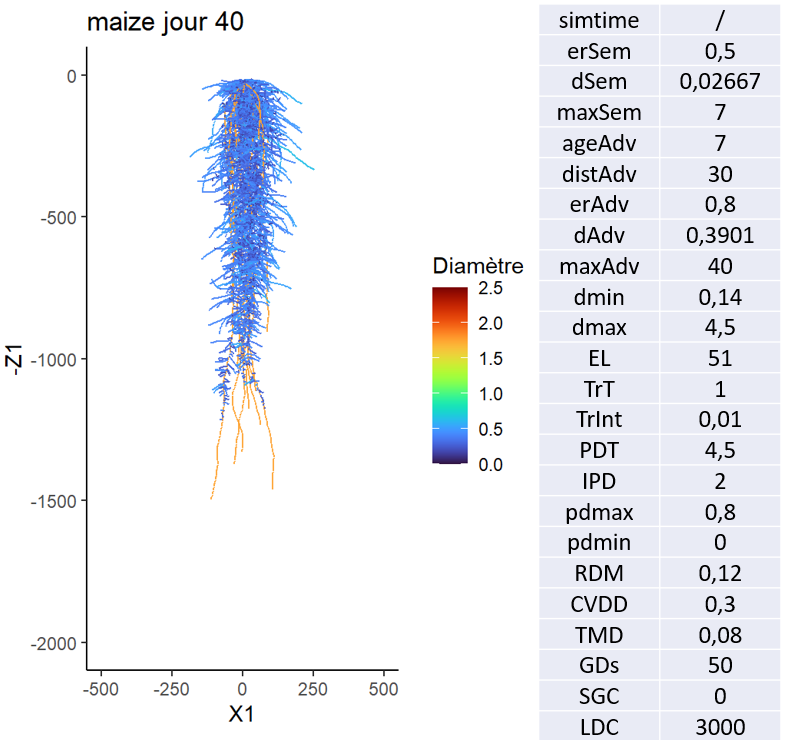
\includegraphics[width=0.6\textwidth]{Image/roots_maize.png}
\caption{Modélisation et paramètres maïs}
\label{fig:roots_maize}
\end{figure}

Le système racinaire alors créer est moins étendu que ceux synthétiser pour le sorgho.
Cette modélisation du maïs donne une profondeur maximale de 1.492 mètres, une largeur de 0.432 mètre et un diamètre moyen de 0.572 mm.
Ces trois valeurs sont chacune plus faibles que celles observées lors des précédentes modélisations de sorgho.
La profondeur atteinte n'est que faiblement inférieure au sorgho, mais les systèmes racinaires produit pour le sorgho couvre une plus grande distance horizontale.
Cette différence vient, d'une part, par des racines adventives qui s'étendent de façon plus verticale chez le maïs et, d'autre part, par les racines latérales qui ont une croissance plus importante chez le sorgho.
\newline

Si on observe bien un système racinaire plus étendu et dense chez le sorgho comme cela est souvent suggéré, il était attendu que les différences de profondeurs soient plus importantes.
Les racines de grands diamètres chez le sorgho devraient, au vu des paramètres observés et des processus du modèle, avoir une élongation bien plus importante que celle du maïs.
Le fait que cela ne soit pas observable peut, en partie être dû à l'estimation de certains paramètres mais il est fortement probable que le fait que les racines adventives sont émises avec le même diamètre engendre en partie ce constat.

\subsubsection{Les échantillons}

Les mesures ayant servi pour estimer les différents paramètres de ArchiSimple proviennent de sources variées.
Certaine sont faites sur des plants de sorgho de fin de culture en champ, d'autre en début de culture en rhizotron et d'autres encore proviennent de sources bibliographiques.
Ces différentes sources vont de pair avec différentes conditions de cultures, différents matériels et différentes méthodes de mesures pouvant influencer les résultats. 
Travailler avec le vivant implique constamment une partie stochastique dans les résultats dû aux éléments imprévisible que conserve les plantes.
Néanmoins, il est possible que les différentes mesures aient été influencés de façon significative par les conditions de culture des plants et les méthodes de mesure.
Cette affirmation est d'autant plus adaptées dans le cadre de ce travail étant donnés que de nombreuses différences sont identifiables dans les conditions de cultures.
En effet, plusieurs différences de traitements sont identifiables entre les échantillons de fin et de début de culture :
\begin{itemize}
    \item Les échantillons en champs ont été confrontées à la compétition, aux aléas climatiques, aux organismes des sols, ... alors que les plants en rhizotron sont maintenus en conditions contrôlées d'humidité, de températures et de lumière.
    \item La présence de champignons au sein des dispositifs en début de culture et l'application du fongicide.
    \item Le milieu dans lequel évolue les racines (perlite vs terre) et les contraintes physiques, biologiques et chimiques qui en découlent.
    \item La nutrition de la plante qui était contrôlée en début de culture et non en champs.
\end{itemize}
Ces nombreux facteurs ont sans aucun doutes affecté le développement de la plante avec une intensité difficilement quantifiable.


\subsubsection{Archisimple }
\citep{pages_modelling_2014-1} (paramètre non exploré par le modèle). \\

ArchiSimple est un modèle plutôt original dans sa façon d'appréhender l'architecture d'un système racinaire.
Les différents processus permettant de faire évoluer le modèle semblent capturer l'essentiel du développement de l'architecture racinaire.
Les inputs requis au fonctionnement du modèle représentent également un atout grâce à leur faible nombre et le fait que ces traits architecturaux sont, pour la plupart, relativement facile à mesurer.
Le fait de ne différencier les racines que part leur diamètre offre une certaine versatilité aux processus qui régissent le modèle, offrant ainsi la possibilité de modéliser presque tout type de système racinaire.
De plus, les différentes relations impliquant les diamètres ont pour la plupart le soutien de différentes études validant son impact sur l'intensité des processus du modèle.
ArchiSimple offre ainsi une approche intéressante, aisée et rapide à la construction d'architecture racinaire.
Cependant, il est apparu dans ce travail que ArchiSimple peut être un peu lacunaire sur certains points.
Celui-ci n'avait pas la prétention de pouvoir remplacer d'autres modèles déjà existants mais plutôt de proposer un modèle versatile qui permet la modélisation de quasiment n'importe quel système racinaire sur la base d'un minimum d'input facilement mesurable.
Les lacunes observées pénalisent principalement la modélisation de système racinaire adventif qui est assez restrictive.
\newline

Tout d'abord, et le plus impactant dans le contexte de ce travail, la façon de définir le diamètre des racines adventives ne correspond pas au développement des Poaceae comme le maïs ou le sorgho.
Ces deux plantes, modélisées précédemment dans ce document, présentent une succession de nœuds qui donne lieu à des racines adventives.
Les échantillons récupérés en champs indiquent que le diamètre des racines nodales émises est alors croissant au fur et à mesure que les nœuds apparaissent.
Or, ArchiSimple ne semble attribuer qu'un unique diamètre aux racines adventives, à savoir $Diametre = dMax*dAdv$.
Cela est particulièrement restrictif dans le cas du maïs et du sorgho ou ces racines représentent, a terme, la totalité du système racinaire.
Cet inconvénient a été contourner en calibrant le paramètre dAdv sur le diamètre moyen des racines adventives.
De cette façon, le système racinaire reste cohérent, mais cela éclipse totalement les variabilités qui seraient observable parmi les diamètres racinaires.
Les premières racines, normalement plus fine, bénéficie de plus de temps pour s'étendre alors que les racines plus jeunes devrait bénéficier d'une vitesse de croissance plus importante au vu de leur diamètre plus important et cela n'est pas du tout pris en compte.
Il résulte alors que des racines avec un diamètre moyen sont émises dès le début développement racinaire et celle-ci atteigne des longueurs trop importantes.
Il serait intéressant d'introduire un paramètre évaluant l'évolution du diamètre des racines adventives en fonction du moment de leurs émissions.
\newline

Ensuite, on retrouve dans ce travail une incohérence entre les paramètres du modèle Dmin et EL.
Ce constat est probablement biaisé par le fait que les échantillons sur lesquels sont calculés EL sont des racines primaires ayant évoluées en rhizotron alors que Dmin provient de racines latérales observées sur des échantillons cultivés en champs.
Néanmoins, les différentes modélisations font face à une dualité entre ces deux valeurs.
Les racines inférieures à 0.2197 mm ne devraient, selon la régression utilisé pour calculer l'élongation potentiel, plus être sujette à une quelconque élongation.
Pourtant, le modèle maintient le processus d'élongation jusqu'au diamètre minimum Dmin qui est bien plus faible (0.1297 ou 0.1567 mm) et qui observerait, selon la régression de EL, une élongation négative.
Cela mène à la conclusion que l'élongation potentielle ne devrait pas être linéaire avec les diamètres.
\newline

En effet, le paramètre EL, considérer comme étant linéaire, n'a pas été observé comme tel par \cite{pellerinand_evaluation_1994}.
Dans le cas présent (et probablement courant) ou celui-ci est estimé sur base de racine de diamètre assez faible, cela pousse la relation du processus d'élongation $PER = EL*D$ (simplification de l'équation \ref{eq:PER}) a estimés une élongation potentielle bien trop importante pour les racines avec des diamètres plus importants.
En outre, la croissance devrait ralentir avec l'âge et la profondeur de la racine tel qu'observer par \cite{pellerinand_evaluation_1994}.
Plusieurs hypothèses justifie cette diminution de l'élongation racinaire.
Cela pourrait provenir du fait que de moins en moins de carbohydrates sont acheminés au plus on s'éloigne des parties aériennes, ou encore des conditions physiques et chimiques rencontrée plus en profondeur.
\newline

Il y a également un problème dans la durée de croissance.
Des simulations de 60 jours engendrent des systèmes racinaire qui s'étendent à plus de trois mètres ce qui est largement supérieur à ce qui serait observé en réalité.
Le paramètre GDs est trop élevé dans notre cas tant pour le sorgho que le maïs.
Ce paramètre mériterait donc d'être estimer à nouveau afin pouvoir limiter la croissance racinaire.
\cite{cahn_relationship_1989} identifie par ailleurs une durée de croissance (GD) différente pour les racines latérales qui ne pourrait pas s'expliquer sur la seule base de leurs diamètres comparé aux autres racines.
\newline

Finalement, une question s'est posée à plusieurs reprises au cours de ce travail de la possibilité de travaillé à l'aide de °Jour comme échelle de temps.
Cette échelle de temps est déjà largement utilisée pour caractériser la croissance aérienne des plantes et son utilisation pour induire l'évolution du système racinaire permettrait la prise en compte de l'environnement de la plante ainsi que ses besoins propres en températures pour se développer.
Plusieurs études lient le développement racinaire au développement aérien, lui-même souvent quantifier en °Jour ce qui a parfois pu complexifier l'estimation des paramètres.
\cite{pellerinand_evaluation_1994} a pareillement identifié un lien entre les températures et le développement du système racinaire.

\subsection{Commentaire sur le sorgho}

Si les printemps secs et les étés déficitaires en eau incitent aux cultures de sorgho, il est encore prématuré de considérer le sorgho comme un candidat pour de grandes cultures en Belgique.
La sélection variétale ne permet pas à ce jour d'assurer qu'une culture de sorgho arrive à terme sans aucun problème.
En effet, le maïs, qui a l'avantage d'être moins exigeant en températures que le sorgho, conserve des rendements plus intéressant à ce jour dans des régions où l'on peut encore observer des années plus fraiches.
L'amélioration et la sélection végétale, encore susceptible à de nombreux progrès pour le sorgho, pourraient permettre d'élargir la gamme de conditions climatiques adaptées à cette culture.
Néanmoins, les trajectoires climatiques promises actuellement pourraient en faire une alternative incontournable dans les régions ou le maïs souffrirait de manque d'eau.
Il pourrait également s'imposer, à une échelle plus modérée, dans des pays comme la Belgique si ses rendements viennent à concurrencer ceux du maïs tout en étant plus résilient.
\newline

Le sorgho conserve tout de même un intérêt particulier dans la recherche.
Il existe encore certains mécanismes participant à sa résilience, pour le moment hors du commun, qui peuvent être identifiés et analysés.
Ces traits peuvent alors participer à orienter la sélection génétique d'autres cultures dans une optique de résilience en réponses aux changements climatiques.

\subsection{Perspective}

L'architecture du système racinaire n'est qu'une étape dans un pipeline permettant de modéliser et de comprendre l'absorption d'eau racinaire et les flux hydriques au sein des plantes.
Les résultats de ArchiSimple est dès lors conçu pour être utilisé par autre modèle permettant d'ajouter une nouvelle dimension qui influence les flux hydriques.
L'architecture générée pourrait par exemple, conjointement avec, entre autre les conductivités axiale et radiale, servir d'input au modèle MARSHALL pour obtenir l'architecture hydraulique du système racinaire.
Les résultats de modélisation obtenus lors de ce travail ne représentent donc pas une fin en soi, mais bien un pas dans un pipeline.
\newline

Les modélisations présentées dans ce travail sont cohérentes, mais semblent omettre beaucoup de caractéristiques de l'architecture racinaire du sorgho, notamment dans le développement de celle-ci.
Il serait dès lors adéquat d'estimer plus précisément les paramètres qui n'ont pas pu être observés sur les échantillons récupérer.
Ces paramètres demandent d'autres expériences assez variées afin d'estimer ces paramètres plus difficilement observables.
\newline

Pour finir, le modèle lui-même est contraignant pour pouvoir représenter un système racinaire fasciculée construit sur des racines adventives comme le sorgho ou le maïs.
ArchiSimple parais intéressant et est déjà très versatile pour construire bon nombre de systèmes racinaires, mais il est nécessaire d'améliorer le processus d'émissions de racines adventives.
Ce processus occupe une place centrale pour les systèmes racinaires considérés dans ce travail et le fait qu'il ne considère qu'un seul diamètre a des répercussions qui se sont avérées critiques dans le modèle.
Le processus d'émission de racines adventives pourrait être amélioré en permettant une augmentation progressive des diamètres des racines adventive émises.
Cette augmentation pourrait se faire sur base du nombre de racines déjà émises, du diamètre de la racine primaire et de Dmax.
Il serait alors possible d'ajouter une équation similaire à l'équation \ref{eq:adv} sans avoir recours à un input supplémentaire pour le modèle.
\begin{equation}
    \begin{gathered}
        dprim = dmax*dsem \\
        dAdv = dprim + \frac{dmax - dprim}{maxAdv}*nAdv
    \end{gathered}
    \label{eq:adv}
\end{equation}
Avec :
\begin{itemize}
    \item dprim : le diamètre de la racine primaire (i.e. dmax*dsem dans ArchiSimple)
    \item dAdv : le diamètre de la racine adventive émise
    \item nAdv : le nombre de racines déjà émises
\end{itemize}
dAdv serait alors calculé au sein du modèle et ne serait plus nécessaire en input.
La première racine adventive aurait dans ce cas un diamètre proche de celui observé sur la racine primaire et augmenterait linéairement avec le nombre d'adventives déjà émise pour, a terme, atteindre dmax.
Toutefois, cette proposition convient à toutes les espèces si deux conditions sont remplies. 
La première est qu'il faut effectivement observer une augmentation des diamètres de racines adventives.
La seconde est qu'il faut que le diamètre maximal soit observé sur une racine adventive.
